\chapter{Binomial Tree Methods}

\section{Background}

As the solutions to the optimal stopping problem do not have a closed form, we would require a benchmark for our numerical results for the different methods we are trying later in the study. We will utilise binomial trees for this for their simplicity and efficiency (it has time complexity $\mathcal O(n^2)$). It works by simulating all possible price paths given some modelling simplifications, and computing the price of the derivative using the martingale property with backwards induction.

To price an American put option with a binomial tree, we will use the binomial discrete-time model. This is an abstraction of the market dynamics, where the stock price can only move to one of two possible new prices in a time step.

To formalise this, let’s fix a time horizon $T > 0$. For some depth $n \ge 1$, divide the interval $[0, T]$ into $n$ even steps each of length $\Delta t = T/n$. The financial market will consist of
\begin{itemize}
    \item A risk-free asset $B_t$ which satisfies
    $$
    B_{i+1} = B_i e^{r\Delta t} \qquad B_0 = 1
    $$
    where $r$ is the continuously-compounded risk-free rate, typically considered interest.
    \item A risky asset $S_t$ which follows a multiplicative binomial evolution:
    
    $$
    S_{i+1} = \begin{cases}
    S_i u & \text{with probability }p \\S_i d & \text{with probability }1-p
    \end{cases}\qquad S_0 > 0
    $$
    
    Here $u$ and $d$ are the model parameters determining the up and down factors of the stock price change per step, where we choose $u > 1$ and $d \in (0,1)$. For an arbitrage free market, we should additionally ensure that
    
    $$
    u > e^{r\Delta t} > d
    $$
    
    for sufficiently small $\Delta t$.
\end{itemize}

For the absence of arbitrage, we require the discounted asset price to have zero drift (admitting a martingale measure). More precisely, let the discounted price be

$$
\tilde S_i = e^{-ri\Delta t} S_i
$$

We require some probability measure $\mathbb Q$, equivalent to the physical measure $\mathbb P$ (have the same non-zero support) such that

$$
\mathbb E_\mathbb Q [\tilde S_{i+1} | \mathcal F_i] = \tilde S_i
$$

To calculate the risk-neutral probability, we can apply this to our model:

$$
e^{-r(i+1)\Delta t}\big[pS_i u + (1-p)S_i d \big] = e^{-ri\Delta t}S_i
$$

Collect the $p$ terms and cancel out the discount factor to get

$$
p(S_i u - S_i d) + S_i d = e^{r\Delta t} S_i
$$

Divide both sides by $S_i$ and rearrange to make $p$ the subject to obtain

$$
p = \frac{e^{r \Delta t} -d}{u-d}
$$

which we will use in our binomial model.

We will adopt a backward induction approach to price the American put at time $0$, since we already know the price at maturity, which is simply the payoff $g: \mathbb R^+ \to \mathbb R$ of the put option:

$$
g(S_T) = (K - S_T)^+
$$

As the discounted price process is a martingale under the risk-free measure $\mathbb Q$, the arbitrage-free value $V_i$ of the derivative at time $i \Delta t$ is necessarily

$$
V_i = \underbrace{e^{-r(T-i\Delta t)}}_\text{discount} \,\mathbb E_\mathbb Q[g(S_T)\,|\,\mathcal F_i]
$$


\section{Implementation}

We will utilise the Cox-Ross-Rubinstein (CRR) Model \cite{cox1979option} for our implementation, which chooses the parameters

$$
u = e^{\sigma \sqrt{\Delta t}}\qquad d = e^{-\sigma \sqrt{\Delta t}}
$$

satisfying the arbitrage free condition, and normalising the local variance of returns to the volatility parameter $\sigma^2$. They also conveniently multiply to $1$.

To implement this, we need to first compute the price tree. This would be, for the price at step $i$ after $j$ up-moves (so clearly $i \ge j$)

$$
S_{i, j} = S_0 u^j d^{i-j}
$$

As the payoff is known at maturity, we can simply set

$$
V_n(j) = g(S_{n, j}) \qquad 0 \le j \le n
$$

and recursively set

$$
V_i(j) = e^{-r\Delta t} \big(p^* V_{i+1}(j+1) + (1-p^*)V_{i+1}(j)\big)
$$

for $0 \le j \le i$. This would be it for European options, but since early exercise is allowed, we will compare this value with the payoff of the price at step $i$ with $j$ up-moves, which is just $f(S_{i, j})$. Thus the value is given by

$$
V_i(j) = \max\bigg(e^{-r\Delta t} \big(p^* V_{i+1}(j+1) + (1-p^*)V_{i+1}(j)\big), \; g(S_{i, j})\bigg)
$$

The root value $V_0(0)$ would be the arbitrage-free option price.

\section{Visualisation}

We are now ready to visualise our binomial tree model. Figure \ref{fig:tree_plot1} plots the option values across different asset prices and different times. We can see that at $t=1$, we are at expiry and hence the value is just the intrinsic value. However, the further we are from expiry, the more the option is worth. This is because the option has time value: the more time we have left to expiry, the more optionality we have and the more opportunity the asset has to be in the money. This additional optionality costs, and hence we can see that the put option loses value over time even if the asset price stays the same.

This phenomenon can be examined more closely in \ref{fig:tree_plot2}. We examine the structures for in the money, at the money and out of the money put options. We supply the European price for reference, and we can see that the European price indeed bounds the American price from below as we'd expect. We can see that the option loses value as we approach maturity. An interesting figure to examine is the in the money figure: we can see that the value flattens at $0.1$, the intrinsic value of the option, at some time $t^\star \in (0, 1)$. This is the point of time beyond which it is always beneficial to perform early exercise, and hence the value of the option is just the intrinsic value. At times $0<t < t^*$ the option is worth more as we have the option to wait, giving the option time value.

\begin{figure}[ht!]
    \centering
    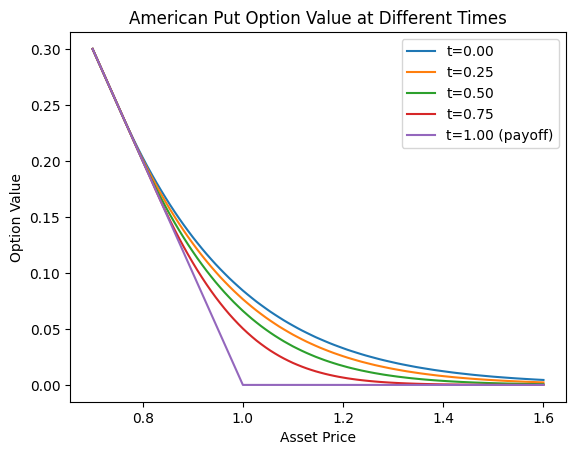
\includegraphics[width=0.5\textwidth]{figures/tree_plot1.png}
    \caption{Option value on different asset prices across time}
    \label{fig:tree_plot1}
\end{figure}

\begin{figure}[ht!]
    \centering
    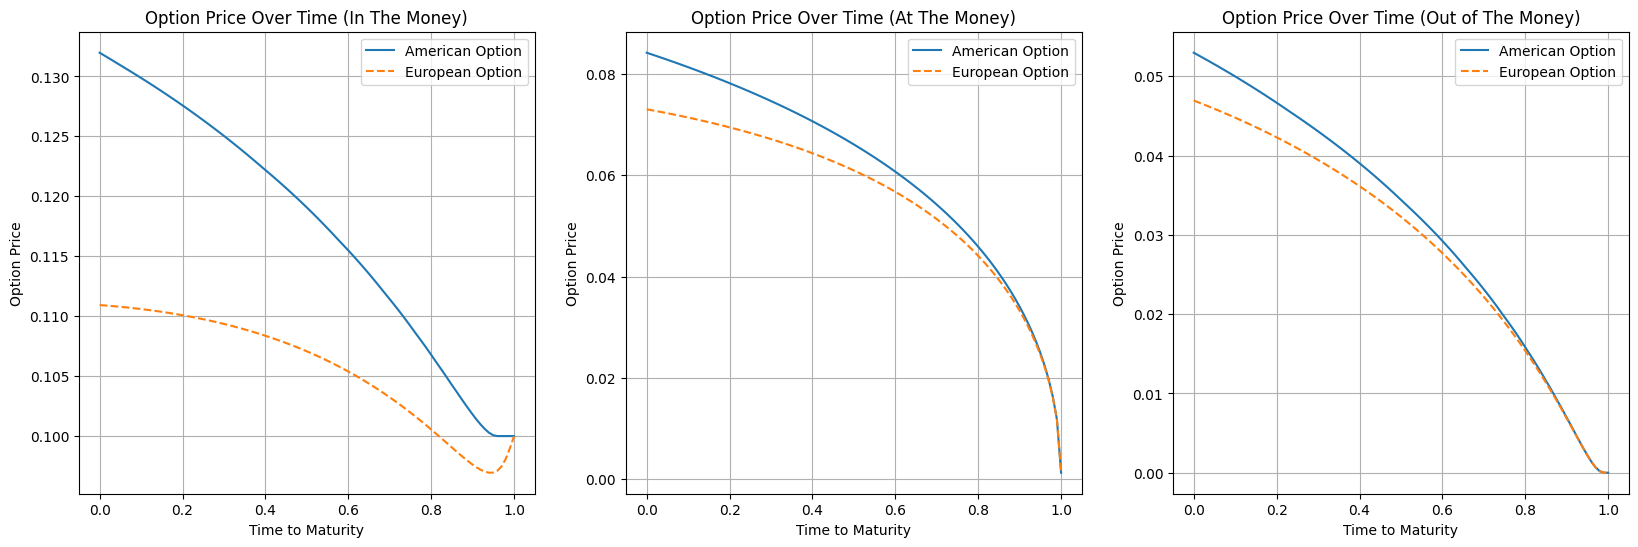
\includegraphics[width=\textwidth]{figures/tree_plot2.png}
    \caption{Decay in time value}
    \label{fig:tree_plot2}
\end{figure}
